
\documentclass[letterpaper, 11pt]{article} 

\usepackage{graphicx} % Paquete necesario para incluir imágenes.
\usepackage{parskip} % Permite configurar formato de párrafos.
\usepackage{amsmath} % Paquete necesario para incluir algunos símbolos matemáticos.
\usepackage{multirow} % Permite agregar algunos elementos de formato a las tablas.
\usepackage[spanish,es-nodecimaldot]{babel} % Permite escribir usando caracteres de la lengua española.
\usepackage[utf8]{inputenc} % Permite escribir usando caracteres de otras lenguas.

\RequirePackage{geometry} % Estas dos instrucciones sirven para modificar las dimensiones de los márgenes.
\geometry{margin=1.9cm}

\selectlanguage{spanish} % Traduce al español subtítulos predeterminados tales como Resumen y Referencias.
\setlength{\parskip}{0.2cm} % Define el espacio entre párrafos.
\setlength{\parindent}{0pt} % Define el tamaño de la sangría en cada párrafo.


%----------------------------------------------------------------------------------------
%	CARÁTULA
%----------------------------------------------------------------------------------------


\title{notas} % Título

\author{YAMIL} % Nombre del autor

\date{\small 22 de mayo de 2019} 

\begin{document}

\maketitle % Crea el título con los datos anteriores

\section*{4.4 Secciones transversales y elementos de matriz. }
Aunque en las secciones anteriores hemos considerado esparcimiento únicamente ondas electromagnéticas incidentes polarizadas en la dirección x, el campo de esparcimiento para luz con una polarización lineal arbitraria y por lo tanto también con un estado de polarización cualquiera \footnote{A partir de la polarización lineal se puede construir la polarización circular y elíptica.}, se obtiene de la simetría de la partícula.

\begin{figure}[hbt]
\centering
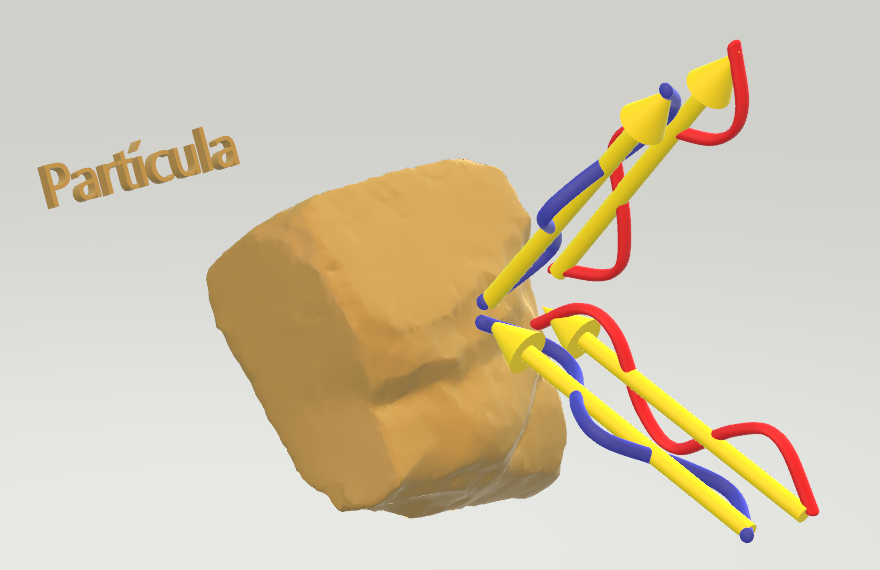
\includegraphics[width=.6\textwidth]{esparcidocualquiera.png}
\caption{Partícula pequeña sin simetría.}
\label{Fig 4.4}
\end{figure}

\textbf{Por ejemplo} relacionamos los campos eléctricos de esparcimiento con igual amplitud pero una polarizada en dirección $x$ y otra en $y$ como:\footnote{Las flechas indican polarización en $x$ y $y$ respectivamente}
\begin{equation}
    \vec{E_{esparcimiento}}(\Phi,\xrightarrow{})=\vec{E_{esparcimiento}}(\Phi+\frac{\pi}{2},\uparrow)
\end{equation}

\begin{figure}[hbt]
\centering
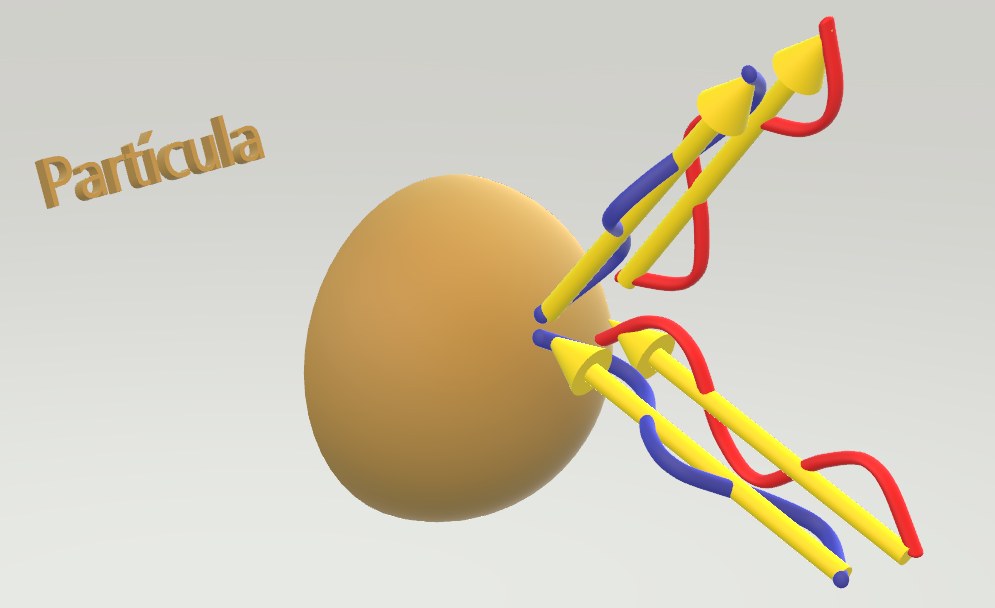
\includegraphics[width=.6\textwidth]{esparcidoesfera.png}
\caption{Partícula pequeña con simetría esférica.}
\label{Fig 4.4}
\end{figure}

Por lo cual como en la sección anterior obtuvimos los coeficientes del campo de esparcimiento $a_n$ y $b_n$ ahora es posible determinar las secciones transversales y la matriz de esparcimiento.
\subsection*{4.4.1 Secciones Transversales.}
Recordando las expresiones de la sección 3.4 para el vector de Poynting:
\begin{equation}
    \vec{S}=\frac{1}{2}Re \left ( \vec{E} \times \vec{H^*}\right) = \frac{1}{2}Re \left( (\vec{E_{inci}+E_{esp}}) \times \vec{(H_{inci}+H_{esp})^*} \right)
\end{equation}
\begin{equation}
    \vec{S}=\frac{1}{2}Re \left ( \vec{E_{inci}} \times \vec{H_{inci}^*}+\vec{E_{esp}} \times \vec{H_{esp}^*}+\vec{E_{inci}} \times \vec{H_{esp}^*}+\vec{E_{esp}} \times \vec{H_{inci}^*}\right)
\end{equation}
Asi podemos relacionar cada termino de la siguiente manera: $\vec{S}=\vec{S_{inc}}+\vec{S_{esp}}+\vec{S_{extinc}}$ donde los dos últimos términos son los que pertenecen al campo de extinción tal que:
\begin{equation}
    \vec{S_{ext}}= \frac{1}{2}Re \left ( \vec{E_{inci}} \times \vec{H_{esp}^*}+\vec{E_{esp}} \times \vec{H_{inci}^*}\right)
\end{equation}
Nuestro objetivo es calcular la energía electromagnética ($W_a$) que cruza una esfera imaginaria centrada en nuestra partícula. con ello es necesario calcular:
\begin{equation}
    W_a= -\int_{esfera} \vec{S} \cdot \vec{da} = -\int_{esfera} \vec{S_i}+\vec{S_{esp}}+\vec{S_{ext}} \cdot \vec{da}=W_i+W_{ext}-W_{esp}
\end{equation}
Suponiendo que el medio en el que se encuentra la partícula es no absorbente $W_i$ será cero. Así mismo $W_a$ no dependerá del radio de nuestra esfera imaginaria, por lo cual podemos hacer la aproximación de campo lejano.
\begin{figure}[hbt]
\centering
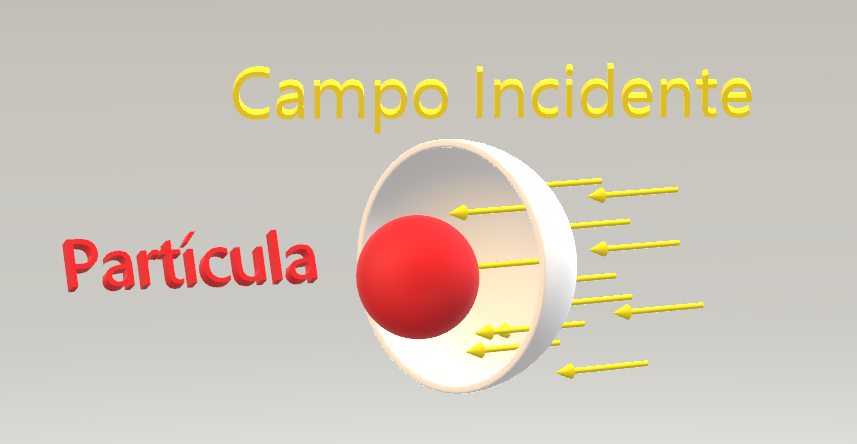
\includegraphics[width=.7\textwidth]{campoincidente.png}
\caption{Esfera imaginaria para el cálculo de la energía electromagnética y el campo incidente.}
\label{Fig 4.4}
\end{figure}
A continuación se derivará una expresión para las secciones transversales de una partícula esférica de manera exacta. Veremos algunas propiedades de las funciones esféricas de Bessel y exploraremos mas el teorema óptico.\\
Cabe mencionar que como se integrará sobre una esfera imaginaria el termino $\vec{da}$ estará en dirección $\vec{e_r}$ por lo cual tenemos que:

\[
(\vec{E_{inc}} \times \vec{H_{esp}})\cdot \vec{da}=
\begin{vmatrix}
da \vec{e_{r}} & 0 & 0   \\ 
E_{inc,r} & E_{inc,\theta} & E_{inc,\phi} \\
H_{esp,r} & H_{esp,\theta} & H_{esp,\phi}  
\end{vmatrix}
=
E_{inc,\theta}H_{esp,\phi}-E_{inc,\phi}H_{esp,\theta}
\]
Recordemos que:
\begin{equation*}
    \vec{E_{inc}}=\sum_{i=1}^{\infty}E_0 \frac{2n+1}{n(n+1)}i^n \left [ \vec{M_{o1n}^{(1)}}-i \vec{N_{e1n}^{(1)}}\right]
\end{equation*}
\begin{equation*}
    \vec{E_{inc}}=\sum_{i=1}^{\infty}E_n\left( E_r\vec{e_r}+ \left [ \cos\Phi \pi_n j_n(\rho)-i(\cos\Phi \tau_n \frac{(j_n(\rho) \rho)^{'}}{\rho}) \right]\vec{e_{\theta}} + \left [ -\sin\Phi \tau_n j_n(\rho)+i(\sin\Phi \pi_n \frac{(j_n(\rho) \rho)^{'}}{\rho}) \right]\vec{e_{\phi}} \right) 
\end{equation*}
\begin{equation*}
    \vec{H_{inc}}=\sum_{i=1}^{\infty}\frac{-E_n k}{\omega \mu}\left( H_r\vec{e_r}+ \left [ -\sin\Phi \pi_n j_n(\rho)+i(\sin\Phi \tau_n \frac{(j_n(\rho) \rho)^{'}}{\rho}) \right]\vec{e_{\theta}} + \left [ -\cos\Phi \pi_n j_n(\rho)+i(\cos\Phi \tau_n \frac{(j_n(\rho) \rho)^{'}}{\rho}) \right]\vec{e_{\phi}} \right) 
\end{equation*}
\begin{equation*}
    \vec{E_{esp}}=\sum_{i=1}^{\infty}E_n\left( E_r\vec{e_r}+ \left [ia_n \cos\phi \tau_n \frac{(h_n(\rho) \rho)^{'}}{\rho} -(b_n\cos\phi \tau_n h_n(\rho) ) \right]\vec{e_{\theta}} - \left [ia_n \sin\phi \pi_n \frac{(h_n(\rho) \rho)^{'}}{\rho}+(b_n\sin\phi \tau_n h_n(\rho)) \right]\vec{e_{\phi}} \right) 
\end{equation*}
\begin{equation*}
    \vec{H_{esp}}=\sum_{i=1}^{\infty}H_n\left( H_r\vec{e_r}+ \left [ ib_n\sin\phi \tau_n\frac{(h_n(\rho) \rho)^{'}}{\rho} -(a_n\sin\phi \pi_n h_n(\rho) ) \right]\vec{e_{\theta}} + \left [ i b_n\cos\phi \pi_n \frac{(h_n(\rho) \rho)^{'}}{\rho}- (a_n \cos\phi \tau_n h_n(\rho)) \right]\vec{e_{\phi}} \right) 
\end{equation*}
Es importante tener en cuenta el siguiente cambio de variable.
\begin{equation}
    \psi_n(\rho)=\rho j_n(\rho) \quad, \quad \xi_n(\rho)=\rho h_n(\rho)
\end{equation}
Ahora podemos escribir las componentes del campo incidente tenemos:
\begin{equation*}
    E_{i,\theta}= \frac{\cos\phi}{\rho}\sum_{n=1}^\infty E_n(\psi_n \pi_n-i\psi_n^{'}\tau_n)
\end{equation*}
\begin{equation*}
    E_{i,\phi}= \frac{\sin\phi}{\rho}\sum_{n=1}^\infty E_n(i\psi_n^{'} \pi_n-i\psi_n\tau_n)
\end{equation*}
\begin{equation*}
    H_{i,\theta}=\frac{k}{\omega \mu}\tan\phi E_{i,\theta} \quad,\quad H_{i,\phi}=\frac{-k}{\omega \mu}\cot \phi E_{i,\phi}
\end{equation*}
Para las componentes del campo esparcido tenemos:
\begin{equation*}
    E_{s,\theta}= \frac{\cos\phi}{\rho}\sum_{n=1}^\infty E_n(ia_n \xi_n^{'} \tau_n-b_n\xi_n\pi_n)
\end{equation*}
\begin{equation*}
    E_{s,\phi}= \frac{\sin\phi}{\rho}\sum_{n=1}^\infty E_n(b_n \xi_n \tau_n-i a_n\xi_n^{'}\pi_n)
\end{equation*}
\begin{equation*}
    H_{s,\theta}=\frac{k}{\omega \mu} \frac{\sin\phi}{\rho}\sum_{n=1}^\infty E_n(i b_n \xi_n^{'} \tau_n- a_n\xi_n\pi_n)
\end{equation*}
\begin{equation*}
    H_{s,\phi}=\frac{k}{\omega \mu} \frac{\cos\phi}{\rho}\sum_{n=1}^\infty E_n(i b_n \xi_n^{'} \pi_n- a_n\xi_n\tau_n)
\end{equation*}
Podemos calcular ahora el trabajo realizado por el campo electromagnético de esparcimiento y de extinción.
\begin{equation}
    W_s=\frac{1}{2}Re\left( \int_0^{2\pi} \int_0^{\pi} (E_{s,\theta}H_{s,\phi}^*-E_{s,\phi}H_{s,\theta}^*)r^2\sin\theta d\theta d\phi\right)
\end{equation}
Desarrollando cada uno de estos términos:
\begin{equation*}
    E_{s,\theta}H_{s,\phi}^{*}=-\frac{\cos^2\phi}{\rho^2}\frac{k}{\omega \mu}\sum_{m=1}^\infty E_n(ia_n \xi_n^{'} \tau_n-b_n\xi_n\pi_n)\sum_{n=1}^\infty E_m^*(ib_m^{*}\xi_m^{{'}^{*}}\pi_m+a_m^* \xi_m^*\tau_m)
\end{equation*}
\begin{equation*}
    -E_{s,\phi}H_{s,\theta}^{*}=-\frac{\sin^2\phi}{\rho^2}\frac{k}{\omega \mu}\sum_{n=1}^\infty E_n(b_n \xi_n \tau_n-ia_n\xi_n^{'}\pi_n)\sum_{m=1}^\infty E_m^*(ib_m^{*}\xi_m^{{'}^{*}}\tau_m+a_m^* \xi_m^*\pi_m)
\end{equation*}
Integrando respecto a $\phi$ primero y recordando que:
\begin{equation}
    \int_0^{2\pi}\sin^2\phi d\phi=\pi=\int_0^{2\pi}\cos^2\phi d\phi
\end{equation}
\begin{equation*}
    W_{esp}=r^2Re\int_0^\pi \frac{\pi k \sin \theta}{\omega \mu \rho^2}\sum_{n,m=1}^\infty E_n E_m^{*}[(a_nb_m^*\xi_n^{'}\xi_m^{'*}\tau_n \pi_m + b_n a_m^{*} \xi_n\xi_m^{*}\pi_n\tau_m+b_na_m^*\xi_n\xi_m^*\tau_n\pi_m
\end{equation*}
\begin{equation*}
    +a_nb_m^*\xi_n^{'}\xi_m^{'*}\pi_n\tau_m)+i(-a_na_m^{*}\xi_n^{'}\xi_m^{*}\tau_n\tau_m+b_nb_m^{*}\xi_n\xi_m^{'*}\pi_n\pi_m-a_na_m^*\xi_n^{'}\xi_m^{*}\pi_n\pi_m+b_nb_m^*\xi_n\xi_m^{'*}\tau_n\tau_m)]d\theta
\end{equation*}
Utilizando las siguientes relaciones:
\begin{equation*}
    \int_0^{\pi}\pi_n \tau_m+\tau_n \pi_m \sin\theta d\theta=\int_0^{\pi}(\frac{P_n^1}{\sin\theta} \frac{dP_m^1}{d\theta}+\frac{P_m^{1}}{\sin\theta}\frac{dP_n^{1}}{d\theta})\sin{\theta}d\theta=
\end{equation*}
\begin{equation*}
    P_n^1(\cos\theta)P_m^1(\cos\theta)|_0^\pi=P_n^1(-1)P_m^1(-1)-P_n^1(1)P_m^1(1)=0
\end{equation*}
Podemos ver este resultado de 
\begin{equation*}
    P_l^m(x)=(-1)^m(1-x^2)^{\frac{m}{2}}\frac{d^m}{dx^m}(P_l(x))
\end{equation*}
Así como:
\begin{equation*}
    \int_0^{\pi}\pi_n \pi_m+\tau_n \tau_m \sin\theta d\theta=\delta_{nm}\frac{2n^2(n+1)^2}{2n+1}
\end{equation*}
\begin{equation*}
    W_{esp}=\frac{\pi}{\omega\mu k}\sum_{n,m=1}^\infty E_nE_m^*Re((a_nb_m^*\xi_n^{'}\xi_m^{'*}+b_na_m^*\xi_n\xi_m^{*})(\int_0^{\pi}\pi_n \tau_m+\tau_n \pi_m \sin\theta d\theta)+
\end{equation*}
\begin{equation*}
    i(a_na_m^*\xi_n^{'}\xi_m^{*}+b_nb_m^*\xi_n\xi_m^{'*})(\int_0^{\pi}\tau_n \tau_m+\pi_n \pi_m \sin\theta d\theta))
\end{equation*}
\begin{equation*}
     W_{esp}=\frac{\pi}{\omega\mu k}\sum_{n,m=1}^\infty |E_o\frac{i^n(2n+1)}{n(n+1)}|^2 Re(-i\xi_n^*\xi_m^{'}|a_n|^2+i\xi_n\xi_m^{'*}|b_n|^2)\frac{2n^2(n+1)^2}{2n+1}
\end{equation*}
\begin{equation}
     W_{esp}=\frac{\pi|E_0|^2}{\omega\mu k}\sum_{n,m=1}^\infty (2n+1) (|a_n|^2+|b_n|^2)
\end{equation}
La ecuación anterior se obtuvo ya que tenemos la siguientes definiciones de las funciones de Riccati-Bessel:
\begin{equation}
    \chi_n=\rho y_n (\rho) \qquad \xi_n=\psi_n - i\chi_n
\end{equation}
Desarrollando la multiplicación de las funciones $\xi_n$ obtenemos:
\begin{equation*}
    -i\xi_n^*\xi_m^{'}=-i(\psi_n^{*}+i\chi_n^{*})(\psi_n^{'}-i\chi_n^{'})=(\chi_n^*\psi_n^{'}-\psi_n^{*}\chi_n^{'})-i(\psi_n^*\psi_n^{'}+\chi_n^{*}\chi_n^{'})
\end{equation*}
\begin{equation*}
    i\xi_n\xi_m^{'*}=i(\psi_n-i\chi_n)(\psi_n^{'*}+i\chi_n^{'*})=(\chi_n\psi_n^{'*}-\psi_n\chi_n^{'*})-i(\psi_n\psi_n^{'*}+\chi_n\chi_n^{'*})
\end{equation*}
Como $\xi_n$ y $\chi_n$ son funciones reales los conjugados se pueden omitir por lo cual de la ecuación diferencial de Riccati-Bessel:
\begin{equation}
    \rho^2\frac{d^2z_n (\rho) }{d\rho^2}+[\rho^2-n(n+1)]z(\rho)=0 \implies W(\rho)=\chi_n\psi_n^{'}-\psi_n\chi_n^{'}=1
\end{equation}
Para calcular la energía de extinción tenemos que resolver la siguiente integral:
\begin{equation}
    W_{ext}=\frac{Re}{2}\left( \int_0^{2\pi} \int_0^{\pi} (E_{i,\phi}H_{s,\theta}^*-E_{i,\theta}H_{s,\phi}^*-E_{s,\theta}H_{i,\phi}^*+E_{s,\phi}H_{i,\theta}^*)r^2\sin\theta d\theta d\phi\right)
\end{equation}
\begin{equation*}
    =\frac{2\pi}{\omega \mu k}\sum_{n=1}^{\infty}(2n+1)Re(a_n+b_n)
\end{equation*}

Obteniendo las secciones transversales de extinción y de esparcimiento obtenidas son:
\begin{equation*}
    C_{esp}=\frac{W_{esp}}{I_{inc}}=\frac{2\pi}{k^2}\sum_{n=1}^{\infty}(2n+1)(|a_n|^2+|b_n|^2)
\end{equation*}
\begin{equation*}
    C_{ext}=\frac{W_{ext}}{I_{inc}}=\frac{2\pi}{k^2}\sum_{n=1}^{\infty}(2n+1)Re(a_n+b_n)
\end{equation*}
Con ello recordamos el teorema óptico el cual nos menciona que la extinción solo depende de la amplitud de esparcimiento en la dirección de propagación.




%----------------------------------------------------------------------------------------
%	REFERENCIAS BIBLIOGRÁFICAS
%----------------------------------------------------------------------------------------

\begin{thebibliography}{99} % Aquí empieza la bibliografía

\bibitem{Ref1} Referencia 1.
.

\end{thebibliography}

\end{document}